 \documentclass{article}
\usepackage{tikz}
\usetikzlibrary{angles, quotes}
\usepackage{amssymb}
\usepackage{pgfplots}
\pgfplotsset{width=10cm,compat=1.9}
\usepgfplotslibrary{statistics}
\usepackage[left=2.54cm,right=2.54cm,top=2.54cm,bottom=2.54cm]{geometry}
\usepackage{tasks} %Paquete necesario para la producción de items horizontales para algunos ejercicios de tarea empleando el comando /begin{multicols}}{#}.../end{multicols} para ayudarnos a reducir las páginas
\usepackage{pdflscape} %comando que permite cambiar a orientación horizontal las hojas%
\usepackage{soul} %Paquete para permitir la compilación de acentos usando el comando {\hl{}}}\\
\sethlcolor{yellow(munsell)} %comando para definir el color para el subrayado usando el comando \hl
\usepackage[utf8]{inputenc}
\usepackage[spanish]{babel}
\usepackage{icomma}
\usepackage{ragged2e}
\usepackage{siunitx}
\usepackage{url}
\usepackage[colorlinks=true, urlcolor=blue,  linkcolor=black, citecolor=green]{hyperref}
\usepackage{pdfpages}
\usepackage{blindtext} %Paquete que genera texto ficticio (dummy text) con el comando: \blindtext
\usepackage{cancel} %in the preamble gives you four different modes of striking through: \cancel{text to cancel} draws a diagonal line (slash) through its argument, \bcancel{text to cancel} uses the negative slope (a backslash), \xcancel{text to cancel} draws an X (actually \cancel plus \bcancel), \cancelto{〈value〉}{〈expression〉} draws a diagonal arrow through the 〈expression〉pointing to the 〈value〉 (math-mode only)
\usepackage{csquotes}
\usepackage{afterpage}
\usepackage{parskip} 
\usepackage{float}
\usepackage{enumitem}
\usepackage{multicol}%Paquete que permite la creación aislada de columnas de texto. De esta forma se reduce la cantidad de páginas en nuestro documento
\usepackage{lipsum} %Paquete que genera texto de relleno al igual que \usepackage{blindtext}, se usa con el comando \lipsum[#-#] los #(hashtags) delimitan el número de páginas que deseamos ocupar del paquete lipsum para usarlos como relleno. 

% Definir el comando personalizado para la nota
\newcommand{\mynote}[1]{%
\begin{tikzpicture}[baseline=-0.75ex]
\node[draw, circle, fill=Apple Green!60, inner sep=2pt] (note) {\textbf{Nota:}};
\end{tikzpicture}%
\ \textit{#1}%
}

\newenvironment{Figura}
{\par\medskip\noindent\minipage{\linewidth}}
{\endminipage\par\medskip}
\usepackage{caption}
\usepackage[
backend=biber,
sorting=none,
url=true
]{biblatex} %bibliografía
\addbibresource{biblio.bib}
% Establecer el espacio entre las entradas de la bibliografía
\setlength{\bibitemsep}{1\baselineskip} % Puedes ajustar el valor según tus preferencias
\usepackage{amsmath,amsthm,amssymb,amsfonts}
\usepackage{pifont} %Permite la compilación del comando \xmark: es el símbolo de la tachita
\usepackage{mathtools} %permite la compilación de símbolos para matrices
\usepackage{empheq} %Paquete que se relaciona con \usepackage[most]{tcolorbox} para la creación de cuadros/cajas de colores para delimitar los resultados matemáticos o líneas de texto usando la línea de comando: \begin{empheq}[box={\mymath[colback=orange(webcolor)!70,drop lifted shadow]}]{equation*} \end{empheq}
\usepackage[most]{tcolorbox} %Paquete que se relaciona con \usepackage{empheq} para la creación de cuadros/cajas de colores para delimitar los resultados matemáticos o líneas de texto
\renewcommand{\qedsymbol}{$\blacksquare$}
\usetikzlibrary{positioning,decorations.pathreplacing} %Paquete que permite la compilación de llaves para cuadros sinópticos (brace diagram) 
\usepackage{schemata} %The schemata package is designed just for these brace diagrams
\usepackage{booktabs}

\newcommand\AB[2]{\schema{\schemabox{#1}}{\schemabox{#2}}} %comando o paquete necesario para crear cuadros sinópticos

\newtcbox{\mymath}[1][]{%
nobeforeafter, math upper, tcbox raise base,
enhanced, colframe=blue!30!black,
colback=blue!30, boxrule=1pt,
#1} %Comando importante para encasillar los resultados matemáticos en cajas de diferentes colores, se relaciona con los paquetes \usepackage{empheq} y \usepackage[most]{tcolorbox} 

\newenvironment{sysmatrix}[1]
{\left(\begin{array}{@{}#1@{}}}
{\end{array}\right)}
\newcommand{\ro}[1]{%
\xrightarrow{\mathmakebox[\rowidth]{#1}}%
}
\newlength{\rowidth}% row operation width
\AtBeginDocument{\setlength{\rowidth}{3em}}  %Comando importante para laproducción de lineas de operaciones entre matrices, método de Gauss o Gauss Jordan se relaciona con \newenvironment{sysmatrix}

%formato para cambiar el horario a español
\usepackage[spanish]{datetime2}
\DTMsetdatestyle{spanish}

\renewcommand{\today}{\DTMdisplaydate{\the\year}{\the\month}{\the\day }{-1}}
%%%%%%%%%%%%%%%%%%%%%%%%%%%%%%%%%%%%%%%%%

\usepackage{datetime}
\newcommand{\mycurrenttime}{\xxivtime}

%%%%%%%%%%%%%%%%%%%%%%%%%%%%%%%%%%%%%%%%%%%%%%%%%%%%%%%%%%%%%%%%%%%%%%%%%%%%%%%%%%%%%%%%%%%%%%%%%%%%%%%%%%%%%%%%%%%%%%%%%%%%%%%%%%%%%%%%%%%%%%%%%


%%%%%%%%%%%%%Caja de color para el título%%%%%%%%%%%%%%%%%%%%%%%%%%%%%%%%%%%%%%%%%%%%%%%%%%%%%%

\definecolor{myframecolor}{RGB}{1, 45, 75} % Prussian Blue
\definecolor{myboxcolor}{RGB}{0, 107, 92} % Apple Green

\newtcolorbox{mybox}{
enhanced,
colback=myboxcolor!7, % Color de fondo del cuadro
colframe=myframecolor, % Color del marco del cuadro
arc=0pt,
boxrule=1pt,
borderline west={2mm}{-10mm}{myframecolor}, % Borde en el lado izquierdo
sharp corners=southwest,
width=\linewidth,
before=\par\vspace{\bigskipamount}, % Espacio antes del cuadro
after=\par\vspace{\bigskipamount} % Espacio después del cuadro
}


\newcommand{\euler}{e} %Comando para producir letra e de euler
\newenvironment{remark}{\par\vfill\footnotesize % Vertical white space above the remark and smaller font size
\begin{list}{}{
	\leftmargin=80pt % Indentation on the left
	\rightmargin=60pt}\item\ignorespaces % Indentation on the right
\makebox[-2.5pt]{\begin{tikzpicture}[overlay]
		\node[draw=Horizon!60,line width=2.5pt,circle,fill=Horizon!25,font=\sffamily\bfseries,inner sep=4pt,outer sep=0pt] at (-19pt,5pt){\textcolor{Horizon}{Nota}};\end{tikzpicture}} % Blue Nota in a circle
\advance\baselineskip -1pt}{\end{list}\vskip5pt} % Tighter line spacing and white space after remark
\usepackage{graphicx}

\usepackage{titling}

\input{colores.tex}

%%Producir signos de cita textual``Asignatura''

\newcommand{\xmark}{\ding{55}} %%%comando que genera la tachita

\newenvironment{MyColorPar}[1]{%
\leavevmode\color{#1}\ignorespaces%
}{%
}%

%%%%%%%%%%%%%%%%%%% Título de la tarea, Nombre de alumno

\title{Clase \#33 - Electrodinámica}
\author{\emph{JA} $\boldsymbol{\mid}$}
\date{\today}

%%%%%%%%%%%%%%%%%%% Datos de la Materia

\usepackage{fancyhdr}
\fancypagestyle{plain}{%  the preset of fancyhdr 
\fancyhf{} % clear all header and footer fields
\fancyfoot[R]{
\includegraphics[width=2cm]{LogoFCFMBUAP (1).png}}
\fancyfoot[L]{{\bfseries{\thedate{}}} a las {\bfseries{\mycurrenttime{}}} horas{} (GMT-6, H. Puebla de Zaragoza, Pue)}
\fancyhead[L]{Electrodinámica}
\fancyhead[R]{\theauthor}
}
\makeatletter
\def\@maketitle{%
\newpage
\null
\vskip 1em%
\begin{center}%
\let \footnote \thanks
{\LARGE \@title \par}%
\vskip 1em%
%{\large \@date}%
\end{center}%
\par
\vskip 1em}
\makeatother

\usepackage{lipsum}  
\usepackage{cmbright}


%%%%%%%%%%%%%%%%%%%%%%%%%%%%%%%%%%%%%%%%%%%%%%%%%%%%%%%%%%%%%%%%%%%%%%%%%%%%%%%%%%%%%%%%%%%%%%%%%%%%%%%%%%%%%%%%%%%%%%%%%%%%%%%%%%%%%%%%%%%%%%%%%%%%%%%%%%%%%%%%%%%%%%%%%%%%%%%%%%%%%%%%%%%%%%%%%%%%%%

\begin{document}



\maketitle


%%%%%%%%%%%%%%%%%%% Datos del profesor, campus y aula

\begin{mybox}
\noindent\begin{tabular}{@{}ll}
	{\bfseries{Profesor}} & Dr. Iván Fuentecilla Cárcamo\\
	\textcolor{prussianblue}{\bfseries{Campus}} / \textcolor{trueblue}{\bfseries{Facultad}}  & \textcolor{prussianblue}{\bfseries{C.U. BUAP}} /  \textcolor{trueblue}{\bfseries{FCFM}} \\
	\textcolor{prussianblue}{\bfseries{Edificio}} /  \textcolor{trueblue}{\bfseries{Salón}}    & 	\textcolor{prussianblue}{\bfseries{EMA4}} /  \textcolor{trueblue}{\bfseries{409}}   
\end{tabular} 
\end{mybox} \vspace{1cm}




	





\begin{MyColorPar}{orange(colorwheel)}

\end{MyColorPar}


\tableofcontents \newpage

\begin{center}
\begin{tikzpicture}
	% Dibuja círculos rellenos en diferentes colores
	\fill[bittersweet] (0,0) circle (0.17cm);
	\fill[Apple Green] (0.6,0) circle (0.17cm);
	\fill[trueblue] (1.2,0) circle (0.17cm);
	\fill[Aguamarina] (1.8,0) circle (0.17cm);
	\fill[Sun] (2.4,0) circle (0.17cm);
	\fill[orange(colorwheel)] (3.0,0) circle (0.17cm);
	\fill[Pesto] (3.6,0) circle (0.17cm);
	\fill[blue-violet] (4.2,0) circle (0.17cm);
	\fill[ticklemepink] (4.8,0) circle (0.17cm);
	\fill[Gallery] (5.4,0) circle (0.17cm);
	\fill[Mantle] (6.0,0) circle (0.17cm);
	\fill[Nevada] (6.6,0) circle (0.17cm);
	\fill[onyx] (7.2,0) circle (0.17cm);
	% Agrega más círculos o modifica los colores según sea necesario
\end{tikzpicture}
\end{center}  \vspace{2cm}




\section{Unit 2: Electric fields in dielectric media}

\begin{figure}[H]
    \centering
	    
\includegraphics[width=0.7\textwidth]{1.png} % ajusta el ancho según convenga
    \caption{Descripción clara y concisa de la figura.}
    \label{fig:mi_figura2}
\end{figure}




Tenemos:

\[ W= \frac{1}{2} \sum\limits_{k=1}^{n}\left(\sum\limits_{j=1}^{n}\right) ^{\prime}\frac{1}{4\pi\epsilon_{0}} \frac{q_{k}q_{j}}{r_{jk}} = \frac{1}{2} \sum\limits_{k=1}^{n}q_{k}U_{k} \]

Con:

\[ r_{kj} = \left|\vec{r}_{k} -\vec{r}_{j}  \right| \]

Tenemos:

\[ U =\left( \sum\limits_{j=1}^{n}\right)^{\prime} \frac{1}{4\pi\epsilon_{0}} \frac{q_{j}}{r_{jk}} \]

In the continuous case,


\[\rho(\vec{r}) \]


\[ \sigma(\vec{r}) \]


\[ 0 \leq \alpha \leq 1 \]


Tenemos:


\begin{equation}
\begin{split}
\left. \begin{array}{cc}
 t & t\mathcal{F}\\
 \alpha \rho(\vec{r}) & \rho(\vec{r})\\
 \alpha \sigma (\vec{r}) & \sigma(\vec{r})
\end{array} \right.  
\end{split} 
\end{equation}


No pasa que al tiempo $t$ en el ejemplo de quitar artpiculos de las personas, esto fue acumulativo, entonces, hacemos un pequeño incremento en la $\alpha$ el cual está relacionado con el tiempo.

La rpegunta es: ¿Cómo relacionariamos el incremento en la carga con el $\delta{\alpha}$?


Tendríamos dos casos, la primera es para el \textbf{caso volumétrico} y el otro caso es el \textbf{caso superficial}. 


Esto es:

$\delta{\alpha}$

\begin{equation}
\begin{split}
\delta{q}\left\{ \begin{array}{cc}
\text{volumetric}\\
\text{superficial}
\end{array} \right.  
\end{split} 
\end{equation}

\section{Unit 2: Electric fields in dielectric media}

\begin{figure}[H]
    \centering
    
\includegraphics[width=0.7\textwidth]{1.png}
    \caption{Descripción clara y concisa de la figura}
    \label{fig:mi_figura2}
\end{figure}

\subsection{Energía electrostática: sistema discreto}
Para $n$ cargas puntuales $\{q_k\}_{k=1}^n$ en el vacío, la energía electrostática total es
\begin{equation}
\label{eq:W_discreto}
W=\frac{1}{2}\sum_{k=1}^{n}\left(\sum_{j=1}^{n}\right)'\frac{1}{4\pi\epsilon_0}\frac{q_k q_j}{r_{jk}}
=\frac{1}{2}\sum_{k=1}^{n} q_k\,U_k
\end{equation}
donde $r_{jk}=\lvert \vec r_j-\vec r_k\rvert$ y $U_k$ es el potencial en la posición de la carga $q_k$ debido a todas las demás cargas
\begin{equation}
\label{eq:Uk_discreto}
U_k=\left(\sum_{j=1}^{n}\right)'\frac{1}{4\pi\epsilon_0}\,\frac{q_j}{r_{jk}}
\end{equation}

\subsection{Paso al continuo}
En el continuo consideramos densidad volumétrica $\rho(\vec r)$ y densidad superficial $\sigma(\vec r)$, que generan un potencial escalar $U(\vec r)$. En medios lineales e isótropos con permitividad efectiva $\epsilon$ (vacío: $\epsilon=\epsilon_0$), el análogo continuo de \eqref{eq:W_discreto} es
\begin{equation}
\label{eq:W_continuo_total}
W=\frac{1}{2}\int_V \rho(\vec r)\,U(\vec r)\,dV \;+\;\frac{1}{2}\oint_S \sigma(\vec r)\,U(\vec r)\,dS
\end{equation}
La expresión \eqref{eq:W_continuo_total} se obtiene rigurosamente con el método de ``cargar'' el sistema mediante un parámetro de homotecia de carga, como se detalla enseguida.

\subsection{Protocolo de carga con un parámetro \texorpdfstring{$\alpha$}{alpha}}
Introducimos un parámetro $\alpha\in[0,1]$ que escala \emph{toda} la distribución de carga desde $0$ hasta su valor final. En cada $\alpha$ tenemos
\begin{equation}
\label{eq:escala_alpha}
\rho_\alpha(\vec r)=\alpha\,\rho(\vec r),\qquad
\sigma_\alpha(\vec r)=\alpha\,\sigma(\vec r)
\end{equation}
En un medio lineal, el potencial responde linealmente a la fuente, por lo que
\begin{equation}
\label{eq:potencial_alpha_lineal}
U_\alpha(\vec r)=\alpha\,U(\vec r)
\end{equation}
donde $U(\vec r)\equiv U_{\alpha=1}(\vec r)$.

La idea física es que el proceso en el tiempo $t$ fue \emph{acumulativo}: al pasar de $\alpha$ a $\alpha+\delta\alpha$ añadimos un pequeño incremento de carga proporcional a $\delta\alpha$. Esto permite computar el trabajo incremental necesario para ``cargar'' el sistema.

\subsection{¿Cómo se relaciona \texorpdfstring{$\delta q$}{delta q} con \texorpdfstring{$\delta\alpha$}{delta alpha}?}
Del escalamiento \eqref{eq:escala_alpha}, los incrementos diferenciales de densidad al pasar de $\alpha$ a $\alpha+\delta\alpha$ son
\begin{equation}
\label{eq:incrementos_densidad}
\delta\rho(\vec r)=\rho(\vec r)\,\delta\alpha,\qquad
\delta\sigma(\vec r)=\sigma(\vec r)\,\delta\alpha
\end{equation}
Por lo tanto, los incrementos de \emph{carga} asociados a un elemento de volumen $dV$ o de superficie $dS$ son
\begin{equation}
\label{eq:deltaq_casos}
\delta q(\vec r)=
\begin{cases}
\delta q_{\text{vol}}(\vec r)=\delta\rho(\vec r)\,dV=\rho(\vec r)\,\delta\alpha\,dV & \text{(caso volumétrico)}\\[4pt]
\delta q_{\text{sup}}(\vec r)=\delta\sigma(\vec r)\,dS=\sigma(\vec r)\,\delta\alpha\,dS & \text{(caso superficial)}
\end{cases}
\end{equation}
La relación clave es, entonces, \(\boxed{\ \delta q \propto \delta\alpha\ }\), con la constante de proporcionalidad dada localmente por la densidad original \(\rho(\vec r)\) o \(\sigma(\vec r)\).

\subsection{Trabajo incremental y energía total}
El trabajo incremental para añadir $\delta q$ cuando el sistema ya está cargado hasta $\alpha$ es
\begin{equation}
\label{eq:deltaW_def}
\delta W(\alpha)=\int_V U_\alpha(\vec r)\,\delta\rho(\vec r)\,dV \;+\;\oint_S U_\alpha(\vec r)\,\delta\sigma(\vec r)\,dS
\end{equation}
Sustituyendo \eqref{eq:potencial_alpha_lineal} y \eqref{eq:incrementos_densidad} en \eqref{eq:deltaW_def}, se obtiene
\begin{equation}
\label{eq:deltaW_alpha}
\delta W(\alpha)=\delta\alpha\left[\alpha\int_V \rho(\vec r)\,U(\vec r)\,dV \;+\;\alpha\oint_S \sigma(\vec r)\,U(\vec r)\,dS\right]
\end{equation}
Integrando \eqref{eq:deltaW_alpha} desde $\alpha=0$ hasta $\alpha=1$,
\begin{equation}
\label{eq:W_integral_alpha}
W=\int_{0}^{1}\delta W(\alpha)
=\left[\frac{\alpha^{2}}{2}\right]_{0}^{1}\left(\int_V \rho\,U\,dV+\oint_S \sigma\,U\,dS\right)
=\frac{1}{2}\int_V \rho\,U\,dV+\frac{1}{2}\oint_S \sigma\,U\,dS
\end{equation}
que coincide con \eqref{eq:W_continuo_total}.

\subsection{Resumen operativo}
\begin{itemize}
\item Al escalar la fuente con $\alpha$ como en \eqref{eq:escala_alpha}, el potencial escala linealmente como en \eqref{eq:potencial_alpha_lineal} en medios lineales
\item El incremento de carga al pasar de $\alpha$ a $\alpha+\delta\alpha$ es localmente \(\delta q_{\text{vol}}=\rho\,\delta\alpha\,dV\) o \(\delta q_{\text{sup}}=\sigma\,\delta\alpha\,dS\) según \eqref{eq:deltaq_casos}
\item El trabajo incremental es \(\delta W(\alpha)=\int U_\alpha\,\delta\rho\,dV+\oint U_\alpha\,\delta\sigma\,dS\) y la integración de \(\alpha=0\) a \(1\) produce el factor \(1/2\) en \eqref{eq:W_integral_alpha}
\end{itemize}

\subsection{Notas sobre medios dieléctricos}
Si el medio es dieléctrico lineal, homogéneo e isótropo, basta reemplazar $\epsilon_0$ por $\epsilon$ donde corresponda y todo el argumento con $\alpha$ se mantiene idéntico, pues la linealidad del problema (relación $U\sim$ fuente) se conserva. En presencia de no linealidades fuertes, $U_\alpha$ ya no escala como en \eqref{eq:potencial_alpha_lineal} y el paso \eqref{eq:W_integral_alpha} debe revisarse
	
	
	
Queremos calcular el trabajo, en su posición, tenemos que tomar en cuenta el potencial que va a tener en el tiempo $t$.

¿Cuál sería el potencial $U^{\prime}(\vec{r}^{\prime})$ en el tiempo $t=0$?

Por ejemplo para poner playeras en algún tiempo $t$ tenemos que considerar reticencia, entonces las teticnecnias también se encuentran en la $U^{\prime}$ en un tiempo $t$.


EN efecto depende del tiempo, si el tiempo transcurre, existen reticencias, entonces si $t=0$, el potencial sería $0$.


Bajo este enfoque, dentro de esta configuracipon total completa a un tiempo $t$.

Nos preguntamos ahora cuál sería el trabajo total ($W_{\text{Total Work}}$)

$\alpha$ es una fracción, i.e. cuando hacemos una prametrización de un trabajo a un tiempo $t$. Cuando hicimos la configuración inicial, el tiempo fue cambiando, entonces el potencial dependía del tiempo y entonces $t$ depende de $\alpha$. Entonces el potencial debería de ir cambiado con respecto a $\alpha$. Así el tiempo lo parametrizamos en forma de $\alpha$. 

Tenemos $\delta{\alpha}$, recordemos que el trabajo es $\Delta{W} = \delta{q}U^{\prime}(\vec{r}^{\prime})$. 


Por ejemplo para:


\[\delta \underbrace{{\rho}}_{contribucion} = \rho \delta{\alpha}  \]

Tendríamos el incremento más toda la contribución, tendríamos entonces:



\[ W = \int\limits_{0}^{1} \rho(\vec{r}^{\prime})\delta{\alpha} U^{\prime}(\alpha,\vec{r}^{\prime}) dv^{\prime} \]


U depende de $\alpha$ y $\vec{r}^{\prime}$ en esta integración tiene que depender de la $\alpha$, es decir el tiempo y de la posición. 

La integral anteerior deberá también tener la parte del volumen:


Es decir: 


\[ W = \int\limits_{V}  \int\limits_{0}^{1} \rho(\vec{r}^{\prime})\delta{\alpha} U^{\prime}(\alpha,\vec{r}^{\prime}) dv^{\prime} \]


Tenemos que el potencial:


\[ U^{\prime} = \alpha U(\vec{r})  \]

Tendríamos nosotros una proporcipon lineal en el potencial respecto al que tenemos en el tiempo $t$. 

EL potencial solo estará cambiando en la intesidad dependiendo de la $\alpha$ particular que nosotros escogamos, dependerá de la distribución de la carga.

En resumen, la proporción anterior el tiempo $t$. 

Introducimos lo anteior y debemos de llegar a la ecuación 6-8. 


Tenemos:

\[   W = \frac{1}{2} \int\limits_{V} \rho(\vec{r}^{\prime})  U(\vec{r}^{\prime}) dv^{\prime} + \frac{1}{2} \int\limits_{S} \sigma (\vec{r}^{\prime}) U(\vec{r}^{\prime}) da^{\prime}   \]

Ahora esto anterior requiere los siguiente comentarios:


\begin{itemize}
\item[$\bullet$] \textbf{Acotado en el espacio}: Esfera suficientemente grande.
\item[$\bullet$] Esta integral será sobre estas superficies conductores.
\end{itemize}

Recordando las superficies equipotenciales nos referimos a putos en ele spacio en donde el potencial tien un valor constante. 


Si tenemos conductoes inmersos cargados dielectricamente, ¿en dónde tendremos una superficie equipotencial?

\textbf{R} = La tendremos en la superficie del conductor.

En la superficie del conductro que está dentro del dielectrico cargado.


Tenemos:


\begin{figure}[H]
    \centering
	    
\includegraphics[width=0.7\textwidth]{2.png} % ajusta el ancho según convenga
    \caption{Descripción clara y concisa de la figura.}
    \label{fig:mi_figura2}
\end{figure}


\textbf{Bounding volumen} y \textbf{surfaces of charge conductors}


Tenemos nosotros: 

\[ W = \frac{1}{2} \int\limits_{V}\rho U(\vec{r}^{\prime})dv + \sum\limits_{j=1}^{n} U_{j} \int\limits_{s_{j}} \sigma(\vec{r}^{\prime})da^{\prime}  \]

\begin{figure}[H]
    \centering
	    
\includegraphics[width=0.7\textwidth]{3.png} % ajusta el ancho según convenga
    \caption{Descripción clara y concisa de la figura.}
    \label{fig:mi_figura2}
\end{figure}

Existe una sumatoria dado que son muchos conductores, la integral de la $\sigma(\vec{r}^{\prime})da^{\prime}$

En la segunda integral tenemos una superficie equipotencial que se podrá factorizar, además no solo tendremos un conductor, sino $n$ conducteos, que en la suoerficie tiene un potencial $q_{1}, q_{2}, \ldots, q_{n}$


El proyecto final consiste en analizar una situación física en la que exista un \textbf{campo electromagnético} en una determinada región del espacio.  
En tal escenario, al \textbf{campo electrostático} podemos asociarle una \textbf{densidad de energía}, mientras que el \textbf{campo electromagnético completo} está vinculado a un \textbf{tensor de energía y momento}.  
A dicho tensor es posible asociarle diversas \textbf{componentes físicas} que describen cómo la energía y el momento se distribuyen y fluyen en el medio.

En las siguientes secciones estudiaremos la \textbf{forma diferencial} de estas expresiones, partiendo del cálculo de la densidad de energía.  
Hacia el final del próximo mes deberemos aplicar estos conceptos de manera concreta, \textbf{calculando explícitamente la densidad de energía del campo electromagnético} en un caso particular.


\begin{figure}[H]
    \centering
	    
\includegraphics[width=0.7\textwidth]{4.png} % ajusta el ancho según convenga
    \caption{Descripción clara y concisa de la figura.}
    \label{fig:mi_figura2}
\end{figure}

Pensemos por ejemplo como obtendríamos la densidad volumetrica de carga sería:


Habíamos visto anteriormente que mediante el vector de desplazamiento eléctrico tenemos:

\begin{equation}
\boxed{
\oint_{S} \vec{D} \cdot d\vec{a} = Q_{\text{libre,\,enc}}
}
\label{eq:gauss_d}
\end{equation}

Esta es la \textbf{forma integral de la ley de Gauss} para medios materiales.  
El campo de desplazamiento eléctrico $\vec{D}$ se define como
\[
\vec{D} = \epsilon_{0}\vec{E} + \vec{P},
\]
donde $\vec{P}$ es la polarización del medio.

La integral de superficie en \eqref{eq:gauss_d} representa el flujo del campo $\vec{D}$ a través de una superficie cerrada $S$,  
y el resultado es igual a la \textbf{carga libre encerrada} dentro del volumen delimitado por esa superficie:
\[
Q_{\text{libre,\,enc}} = \int_{V} \rho_{\text{libre}}\, dV
\]
De este modo, la ley de Gauss en su forma diferencial se expresa como
\begin{equation}
\boxed{
\nabla \cdot \vec{D} = \rho_{\text{libre}}
}
\label{eq:gauss_dif}
\end{equation}


Tenemos que para cualquier volumen la diferncia de integrandos es $0$, entonces implica que:

\[ \rho = \nabla \cdot \vec{D} \]

Determinar que sería la $\sigma(\vec{r})$ a partir del vector de desplzamiento eléctrico. 
 
 
\subsection{Densidad de carga superficial a partir de \texorpdfstring{$\vec D$}{D}}

Partimos de la ley de Gauss macroscópica para el desplazamiento eléctrico:
\begin{equation}
\boxed{\ \nabla\!\cdot\!\vec D=\rho_{\text{libre}}\ }
\label{eq:gaussD}
\end{equation}

Para una \textbf{superficie} $S$ (por ejemplo, una interfaz entre dos medios) usamos una \emph{pastilla gaussiana} y tomamos el límite de su espesor $h\to 0$. La forma integral de \eqref{eq:gaussD} produce la condición de salto en la componente normal de $\vec D$:
\begin{equation}
\boxed{\ \hat{\boldsymbol n}\!\cdot\!\big(\vec D_{2}-\vec D_{1}\big)=\sigma_{\text{libre}}(\vec r_{S})\ }
\label{eq:jumpD}
\end{equation}
donde $\hat{\boldsymbol n}$ es la normal unitaria que apunta de la región $1$ a la región $2$, y $\vec r_{S}$ es un punto sobre la superficie. En particular:

\begin{itemize}
\item \textbf{Conductor–dieléctrico (electrostática):} dentro del conductor $\vec D_{1}=\vec 0$, por lo que
\begin{equation}
\boxed{\ \sigma_{\text{libre}}=\hat{\boldsymbol n}\!\cdot\!\vec D_{\text{fuera}}\ }
\label{eq:sigma_conductor}
\end{equation}

\item \textbf{Interfaz dieléctrico–dieléctrico:} si existe una lámina de \emph{carga libre} en la interfaz, entonces \eqref{eq:jumpD} da directamente esa densidad superficial; si no hay carga libre en la interfaz, \(\sigma_{\text{libre}}=0\) y la componente normal de \(\vec D\) es continua.
\end{itemize}

\paragraph{Cargas ligadas (polarización).}
Si además queremos la \emph{carga superficial ligada} (debida a polarización), recordamos que
\begin{equation}
\boxed{\ \rho_{\text{ligada}}=-\nabla\!\cdot\!\vec P,\qquad
\sigma_{\text{ligada}}=\vec P\!\cdot\!\hat{\boldsymbol n}\ }
\label{eq:bound}
\end{equation}
(en una interfaz entre dos medios polarizados, \(\sigma_{\text{ligada}}=\hat{\boldsymbol n}\!\cdot\!\big(\vec P_{2}-\vec P_{1}\big)\)).

\paragraph{Relación con \texorpdfstring{$\vec E$}{E}.}
Usando \(\vec D=\epsilon_{0}\vec E+\vec P\), separamos cargas libres y ligadas:
\begin{equation}
\hat{\boldsymbol n}\!\cdot\!\big(\epsilon_{0}\vec E_{2}-\epsilon_{0}\vec E_{1}\big)
+\hat{\boldsymbol n}\!\cdot\!\big(\vec P_{2}-\vec P_{1}\big)
=\sigma_{\text{libre}}
\label{eq:split}
\end{equation}
lo que es consistente con \eqref{eq:jumpD} y \eqref{eq:bound}. En medios lineales e isótropos, \(\vec D=\epsilon\,\vec E\), de modo que
\begin{equation}
\boxed{\ \hat{\boldsymbol n}\!\cdot\!\big(\epsilon_{2}\vec E_{2}-\epsilon_{1}\vec E_{1}\big)
=\sigma_{\text{libre}}\ }
\label{eq:linear_media}
\end{equation}

\paragraph{Conclusión práctica.}
La \textbf{densidad de carga superficial libre} se obtiene directamente de \(\vec D\) como el \emph{salto} de su componente normal en la interfaz, \eqref{eq:jumpD}. En un conductor, basta \eqref{eq:sigma_conductor}. Si se requiere la \textbf{carga superficial ligada}, se usa \(\sigma_{\text{ligada}}=\vec P\!\cdot\!\hat{\boldsymbol n}\).

Para lo anterior usamos una \textbf{pillbox}, pero el caso acá es que estamos usando un dielectrico.


\begin{figure}[H]
    \centering
	    
\includegraphics[width=0.5\textwidth]{5.png} % ajusta el ancho según convenga
    \caption{Descripción clara y concisa de la figura.}
    \label{fig:mi_figura2}
\end{figure}

Usando ley de Gauss tenemos que la $\sigma$ tiene la forma anterior.


Tenemos: 

\begin{figure}[H]
    \centering
	    
\includegraphics[width=0.5\textwidth]{6.png} % ajusta el ancho según convenga
    \caption{Descripción clara y concisa de la figura.}
    \label{fig:mi_figura2}
\end{figure}

Siguiente unidad magnetostostatica.

Siguiente a esa es campo dependiente del tiempo.

Tenemos que deducir la relación de la energía en el caso electrostático.



\begin{figure}[H]
    \centering
	    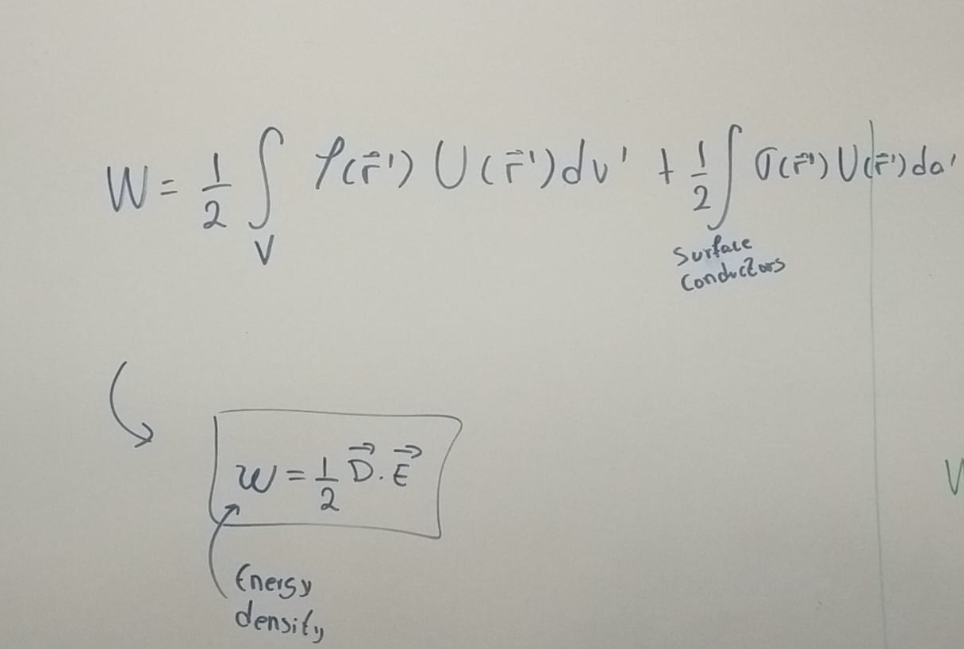
\includegraphics[width=0.5\textwidth]{7.png} % ajusta el ancho según convenga
    \caption{Descripción clara y concisa de la figura.}
    \label{fig:mi_figura2}
\end{figure}


\subsection{De \texorpdfstring{$\rho\,U$}{rho U} a \texorpdfstring{$\vec D$}{D} (paso a paso)}

Partimos de la expresión de energía electrostática (fuente libre distribuida en volumen $V$ y, si aplica, en superficie $S$):
\begin{equation}
\label{eq:W_rho_sigma}
W=\frac{1}{2}\int_V \rho_{\text{libre}}(\vec r')\,U(\vec r')\,dV' \;+\; \frac{1}{2}\oint_S \sigma_{\text{libre}}(\vec r')\,U(\vec r')\,dS'
\end{equation}
donde $U$ es el potencial eléctrico macroscópico. (Los primes indican variables mudas de integración.)

\paragraph{Paso 1: Sustituir \(\rho_{\text{libre}}\) por \(\nabla\!\cdot\!\vec D\).}
Por la ley de Gauss macroscópica,
\begin{equation}
\label{eq:gaussD}
\nabla\!\cdot\!\vec D=\rho_{\text{libre}}
\end{equation}
entonces el término volumétrico de \eqref{eq:W_rho_sigma} queda
\begin{equation}
\label{eq:W_vol_D}
\int_V \rho_{\text{libre}}\,U\,dV'=\int_V \big(\nabla\!\cdot\!\vec D\big)\,U\,dV'
\end{equation}

\paragraph{Paso 2: Identidad vectorial clave.}
Usamos la regla del producto para la divergencia:
\begin{equation}
\label{eq:prod_rule}
\nabla\!\cdot\!\big(U\,\vec D\big)=U\,\nabla\!\cdot\!\vec D+\vec D\!\cdot\!\nabla U
\end{equation}
De \eqref{eq:prod_rule} se despeja
\begin{equation}
\label{eq:U_divD}
U\,\nabla\!\cdot\!\vec D=\nabla\!\cdot\!\big(U\,\vec D\big)-\vec D\!\cdot\!\nabla U
\end{equation}
Sustituyendo \eqref{eq:U_divD} en \eqref{eq:W_vol_D}:
\begin{equation}
\label{eq:int_by_parts_step}
\int_V \big(\nabla\!\cdot\!\vec D\big)\,U\,dV'
=\int_V \nabla\!\cdot\!\big(U\,\vec D\big)\,dV' - \int_V \vec D\!\cdot\!\nabla U\,dV'
\end{equation}

\paragraph{Paso 3: Teorema de la divergencia.}
Aplicando el teorema de Gauss al primer término de \eqref{eq:int_by_parts_step}:
\begin{equation}
\label{eq:gauss_surface}
\int_V \nabla\!\cdot\!\big(U\,\vec D\big)\,dV'=\oint_S U\,\vec D\!\cdot\!\hat{\boldsymbol n}\,dS'
\end{equation}
Por tanto,
\begin{equation}
\label{eq:split_surface_volume}
\int_V \rho_{\text{libre}}\,U\,dV'
=\oint_S U\,\vec D\!\cdot\!\hat{\boldsymbol n}\,dS' - \int_V \vec D\!\cdot\!\nabla U\,dV'
\end{equation}

\paragraph{Paso 4: Relación con el campo eléctrico.}
En electrostática, \(\vec E=-\nabla U\). Entonces
\begin{equation}
\label{eq:DgradU_to_DE}
-\vec D\!\cdot\!\nabla U=\vec D\!\cdot\!\vec E
\end{equation}
y \eqref{eq:split_surface_volume} se convierte en
\begin{equation}
\label{eq:rhoU_to_surface_plus_DE}
\int_V \rho_{\text{libre}}\,U\,dV'
=\oint_S U\,\vec D\!\cdot\!\hat{\boldsymbol n}\,dS' \;+\; \int_V \vec D\!\cdot\!\vec E\,dV'
\end{equation}

\paragraph{Paso 5: Reunir términos de \eqref{eq:W_rho_sigma}.}
Reponiendo \eqref{eq:rhoU_to_surface_plus_DE} en \eqref{eq:W_rho_sigma}:
\begin{equation}
\label{eq:W_mixture}
W=\frac{1}{2}\left[\oint_S U\,\vec D\!\cdot\!\hat{\boldsymbol n}\,dS' + \int_V \vec D\!\cdot\!\vec E\,dV'\right]
\;+\; \frac{1}{2}\oint_S \sigma_{\text{libre}}\,U\,dS'
\end{equation}

\paragraph{Paso 6: Interpretación del término superficial.}
En una superficie portadora de \emph{carga libre} \(\sigma_{\text{libre}}\), el salto de la componente normal de \(\vec D\) satisface
\begin{equation}
\label{eq:jump_D}
\hat{\boldsymbol n}\!\cdot\!\big(\vec D_{2}-\vec D_{1}\big)=\sigma_{\text{libre}}
\end{equation}
De aquí se sigue que el aporte \(\oint_S U\,\vec D\!\cdot\!\hat{\boldsymbol n}\,dS'\) reproduce exactamente el término \(\oint_S \sigma_{\text{libre}} U\,dS'\) cuando se toma el límite de pastilla gaussiana en la interfaz. En consecuencia, ambos términos superficiales se combinan de forma consistente.

\paragraph{Conclusión 1 (forma campo).}
Si no hay aportes superficiales netos (por ejemplo, contorno a infinito con \(U\to 0\) suficientemente rápido, o si la contabilidad de la interfaz ya está incluida vía \(\sigma_{\text{libre}}\)), obtenemos la forma puramente volumétrica
\begin{equation}
\boxed{\
W=\frac{1}{2}\int_V \vec D\!\cdot\!\vec E\,dV'\
}
\label{eq:W_DE}
\end{equation}

\paragraph{Conclusión 2 (medio lineal isótropo).}
En medios lineales e isótropos, \(\vec D=\epsilon\,\vec E\), y \eqref{eq:W_DE} se reduce a
\begin{equation}
\boxed{\
W=\frac{1}{2}\int_V \epsilon\,\lvert \vec E\rvert^{2}\,dV'\
}
\label{eq:W_epsE2}
\end{equation}

\paragraph{Lo pedido en el enunciado.}
En particular, del paso \eqref{eq:U_divD} se ve explícitamente que
\begin{equation}
\boxed{\
U\,\nabla\!\cdot\!\vec D \;=\; \nabla\!\cdot\!\big(U\,\vec D\big)\;-\;\vec D\!\cdot\!\nabla U\
}
\label{eq:UdivD_identity}
\end{equation}
que es la \textbf{forma de divergencia} buscada para el término \(U\,\nabla\!\cdot\!\vec D\). Sustituyendo \(\nabla U=-\vec E\) se conecta con \(\vec D\!\cdot\!\vec E\) como en \eqref{eq:DgradU_to_DE} y \eqref{eq:W_DE}.



\begin{figure}[H]
    \centering
	    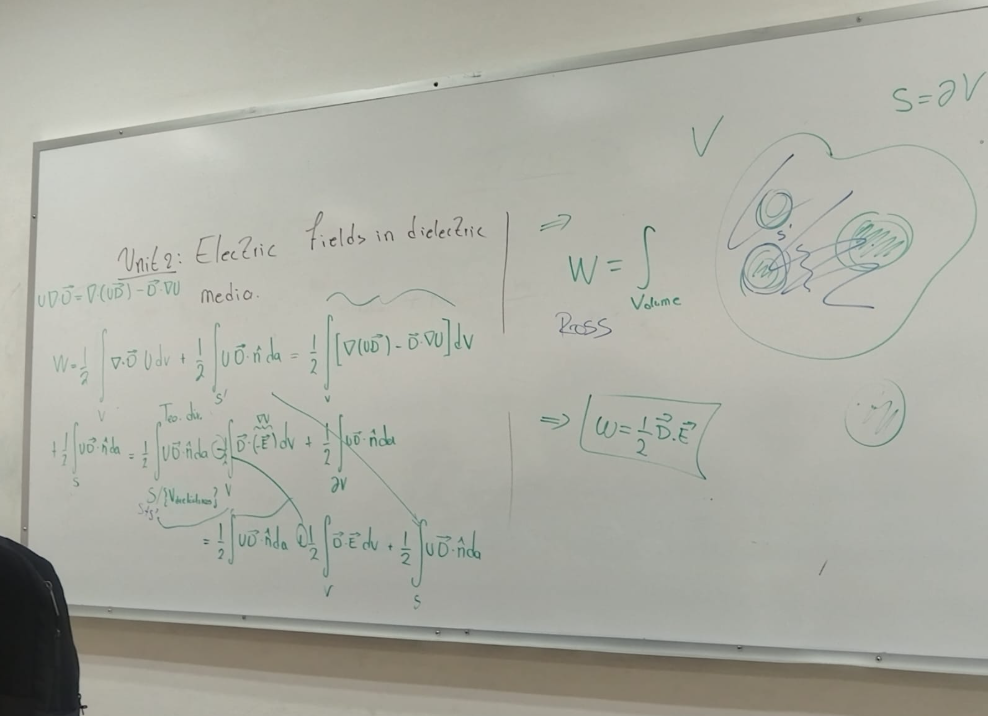
\includegraphics[width=1.1\textwidth]{8.png} % ajusta el ancho según convenga
    \caption{Descripción clara y concisa de la figura.}
    \label{fig:mi_figura2}
\end{figure}




 
\end{document}